\chapter{Rahmenentfernung}

\begin{figure}[h]
 	$
 	G = \frac{1}{159}
	\begin{bmatrix}
		2 & 4 & 5 & 4 & 2 \\ 
		4 & 9 & 12 & 9 & 4 \\
		5 & 12 & 15 & 12 & 5 \\
		4 & 9 & 12 & 9 & 4 \\
		2 & 4 & 5 & 4 & 2 \\
	\end{bmatrix},	
	$
	$
	S_x = 
	\begin{bmatrix}
	-1 & 0 & +1 \\
	-2 & 0 & +2 \\
	-1 & 0 & +1
	\end{bmatrix},
	$
	$	
	S_y = 
	\begin{bmatrix}
	-1 & -2 & -1 \\
	0 & 0 & 0 \\
	+1 & +2 & +1
	\end{bmatrix},
	$
\caption{Die Figur zeigt den Gausfilterkernel sowie die Faltungsmasken des Sobeloperators, die beim Canny-Algorithmus verwendet werden}
\label{fig:gauss}
\end{figure}

Die Extraktion eines Bildes aus einem monotonen Rahmen geschieht in mehreren Schritten. Zu erst werden die Kanten des Bildes detektiert um mit dem daraus resultierenden Binärbild festzustellen, ob sich ein monotoner Rahmen um das eigentliche Bild befindet. 


Zur Detektion von Kanten gibt es mehrere Möglichkeiten, da es aber wichtig ist, dass die Kanten möglichst Pixel genau detektiert werden, ist der Canny-Kantendetektionsalgorithmus am besten dazu geeignet. 
Bei diesem Verfahren wird zu erst rauschen aus dem Bild durch einen Gaußfilter entfernt. Der Kernel für einen 5x5 Gausfilter ist in Abbildung \ref{fig:gauss} dargestellt. 
Mit Hilfe der Sobeloperatoren für die X-, Y-Richtung werden danach die Gradienten des Bildes errechnet. Die dazu benötigten Faltungskerne sind ebenfalls in Abbildung \ref{fig:gauss} dargestellt. 
Mit den so gewonnen Ableitungen kann man dann die Richtung des Gradienten berechnen und die absolute Kantenstärke.
Damit nun jede Kante nicht mehr als ein Pixel breit ist, soll mit Hilfe einer Non-maximum-suppression nur die Maxima entlang einer Kante erhalten bleiben. 
Bei der Non-maximum-suppression wird der Wert eines Pixels der Kante mit den Pixeln rechts und links neben der Kante verglichen. Sollte einer der Werte größer sein wird der betrachtete Pixel auf null gesetzt.
Danach wird noch festgestellt, ab welcher Kantenstärke ein Pixel überhaupt zu einer Kante gehört. Das Ergebniss des Kantendetektionsalgorithmus ist dann ein Binärbild indem jede gefundene Kante mit weißen Pixeln dargestellt ist (\cite{OpenCVCanny}).

Um nun im nächsten Schritt den monotonen Rahmen zu erkennen muss man beachten, dass sich innerhalb des Rahmens keine Kanten befinden, nur zu beginn des Rahmens und direkt danach. Um diese Fläche ohne Kanten zu detektieren wird zuerst ein Bildausschnitt entlang einer der vier Seiten erzeugt. Der Bildausschnitt erstreckt sich über die komplette Seite des Bildes und reicht eine bestimmte Anzahlt an Pixeln in das Bild. Die Tiefe mit der der Ausschnitt in das Bild reicht wird dann Schritt für Schritt vergrößert. In jedem Schritt wird die Anzahl der weißen Pixel innerhalb des Ausschnittes gezählt. 
In Abbildung \ref{fig:bordergradient} kann man die Zunahme der weißen Pixel in den einzelnen Bildausschnitten ablesen.   

\begin{figure}[h]
	\centering
	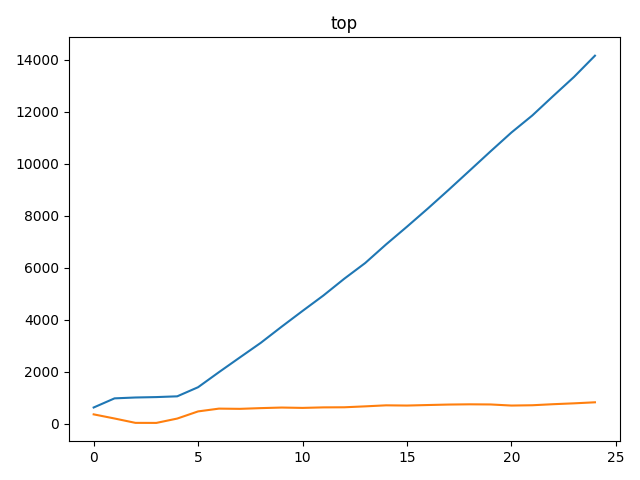
\includegraphics[width=0.3\linewidth]{images/plot_frame/plot_top_frame.png}
	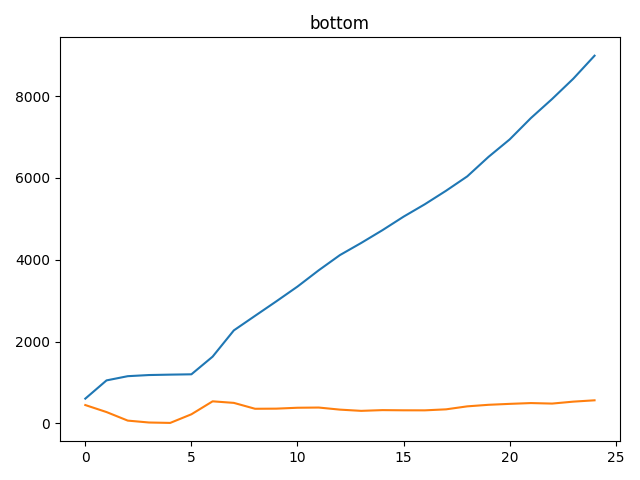
\includegraphics[width=0.3\linewidth]{images/plot_frame/plot_bottom_frame.png}\\
	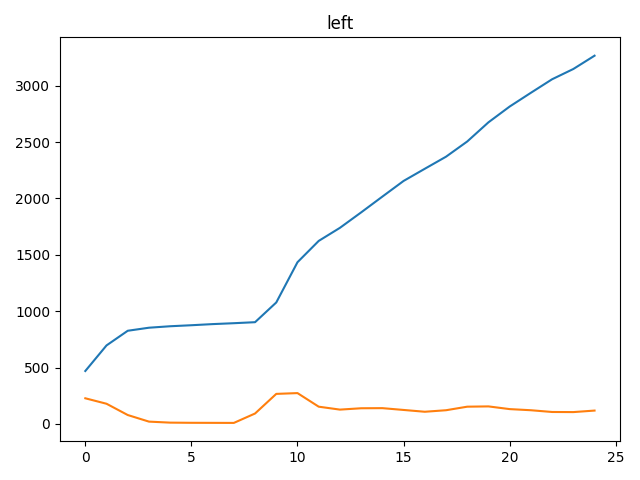
\includegraphics[width=0.3\linewidth]{images/plot_frame/plot_left_frame.png}
	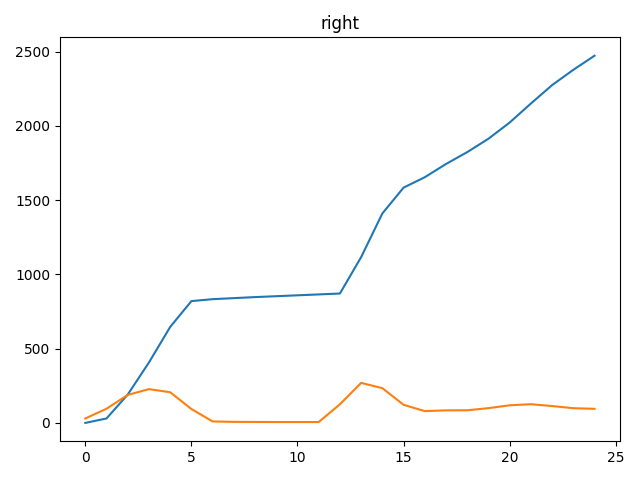
\includegraphics[width=0.3\linewidth]{images/plot_frame/plot_right_frame.png}
	\caption{Die obere Linie zeigt die Zunahme weißer Pixel in den schrittweise größer werdenden Bildausschnitten. Die untere Linie zeigt die Gradient der Zunahme zum vorhergehenden Schritt.}
	\label{fig:bordergradient}
\end{figure}  

Da sich innerhalb des Rahmen kaum weiße Pixel befinden kann man in der Abbildung deutlich sehen das in einem bestimmten Bereich die Anzahl der weißen Pixel fast gleich bleibt. In diesem Bereich muss sich der Rahmen befinden. Direkt danach nimmt die Anzahl deutlich zu. Dies muss der Beginn des eigentlichen Bildes sein. 
Um nun erkennen zu können, wann das eigentliche Bild beginnt wird der Gradient, der Zunahme von weißen Pixeln, verwendet. Dieser ist ebenfalls in der Abbildung \ref{fig:bordergradient} dargestellt. 
Der Gradient ist am geringsten in den Bereichen des Rahmens und hat dann ein kleines Maximum direkt nach dem Rahmen. 

Im nächsten Schritt kann man dann mit Hilfe des davor erzeugten Gradienten das Bild soweit abschneiden, dass kein Rahmen mehr enthalten ist. Dazu sucht man den Schritt an dem der Gradient am kleinsten ist und geht die folgenden Schritte weiter bis zu dem nächsten Maximum. Anhand der Anzahl von Schritten die vom Rand des Bildes bis zum Maximum gegangen wurden kann man die Anzahl an Pixeln bestimmen, die an dieser Seite des Bildes abgeschnitten werden müssen. Sollte kein Maximum gefunden werden oder sollte das Maximum zu weit entfernt sein vom Minimum der Gradienten, dann wird kein Schnitt ausgeführt.